% ******************************* Thesis Appendix B ********************************
\label{ch:app_dphistar}


\chapter{\mindphistar requirement in the signal region}

As described in chapter~\ref{ch:5}, an event level requirement is made in the
signal region such that all events have \mindphistar > 0.3, such that any
remaining QCD MJ contaminated events are removed. This appendix outlines some of
the studies to motivate and characterise this requirement.

\section{Motivation}

The hadronic signal region selection criteria are specifically
designed to remove many orders of magnitude of QCD MJ events, in particular the
use of variables such as \alphat and \mhtmet contribute significantly to this.
However, despite these strict requirements a small fraction of QCD MC events are
observed to still enter into the signal region.

PLOTS OF QCD MC IN SIGNAL REGION

The remaining QCD events are from genuine physics processes, when a jet overlaps
with genuine \met. This missing energy occurs due to heavy flavour mesons in
jets decaying leptonically. Of the lepton and neutrino pair, the neutrino
carries the bulk share of the pair's momentum, leading to soft leptons which
can evade leptonic vetoes and non-negligible amounts of invisible energy. An
event display of a typical event is shown 

show how there is still QCD MC surviving the hadronic selection. can show as a
function of HT or MHT or alphaT or something. MC only!!

how do these events pass alphat and MHTovMET?

what are these events? what do they look like? real physics processes - jets
decaying via neutrinos to give soft leptons and neutrinos carrying significant
amounts of missing energy. this gives a severely mis-measured jet, as a
large fraction of the jet's energy is invisible - met aligned with jet axis.

ultimately used to reject events with genuine missing energy coming from a jet.
heavy flavour mesons decaying leptonically, producing neutrinos. Could even show
an event display and/or event chain.

\section{Isolating these events}

Can isolate these events using a variable defined to look for `mis-measured'
jets that align with met or mht - \mindphistar.

can show the QCD MG MC plots of \dphistar - see peak around zero for QCD, even
after full selection and alphaT cuts. Can show without data...! Still though,
what about the handful of events at higher dphistar?

excess vs QCD alphaT evolution plots - observed excess appears to be QCD-like.
\emph{THIS IS ACKNOWLEDGING AN EXCESS!}

\section{Effect of hadronic region}

\emph{How well does this work?} Very well! Removes all remaining QCD events that
contain missing energy. \emph{What about the remaining few QCD MG events at high
dPhiStar?} can show rob's plots of the dphiStar above/below

\section{Effect on signal models}
we do take a hit, but hopefully equivalent of more so in BG pred, so S/B is
preserved. either way, we have to make the cut, so we deal with the consequence
in terms of signal efficiency.

this cut can be particularly damaging to compressed spectra models where a
soft susy decay is balanced by hard ISR, creating co-linear decay products and
neutralino's. ho-hum.

\emph{How much do we `lose' in signal efficiency?} Show signal efficiency
difference plots, with vs without.

\clearpage
% \begin{figure}
%     \centering
%     \includegraphics[angle=90, width=\textwidth]
%     {Figs/eventDisplays/Had_QCD_MG_MC_HT375_skim_displays_singleEvent.pdf}
%     \caption{Event display blah}
%     \label{fig:event_display_QCD}
% \end{figure}

\begin{sidewaysfigure}
    \centering
    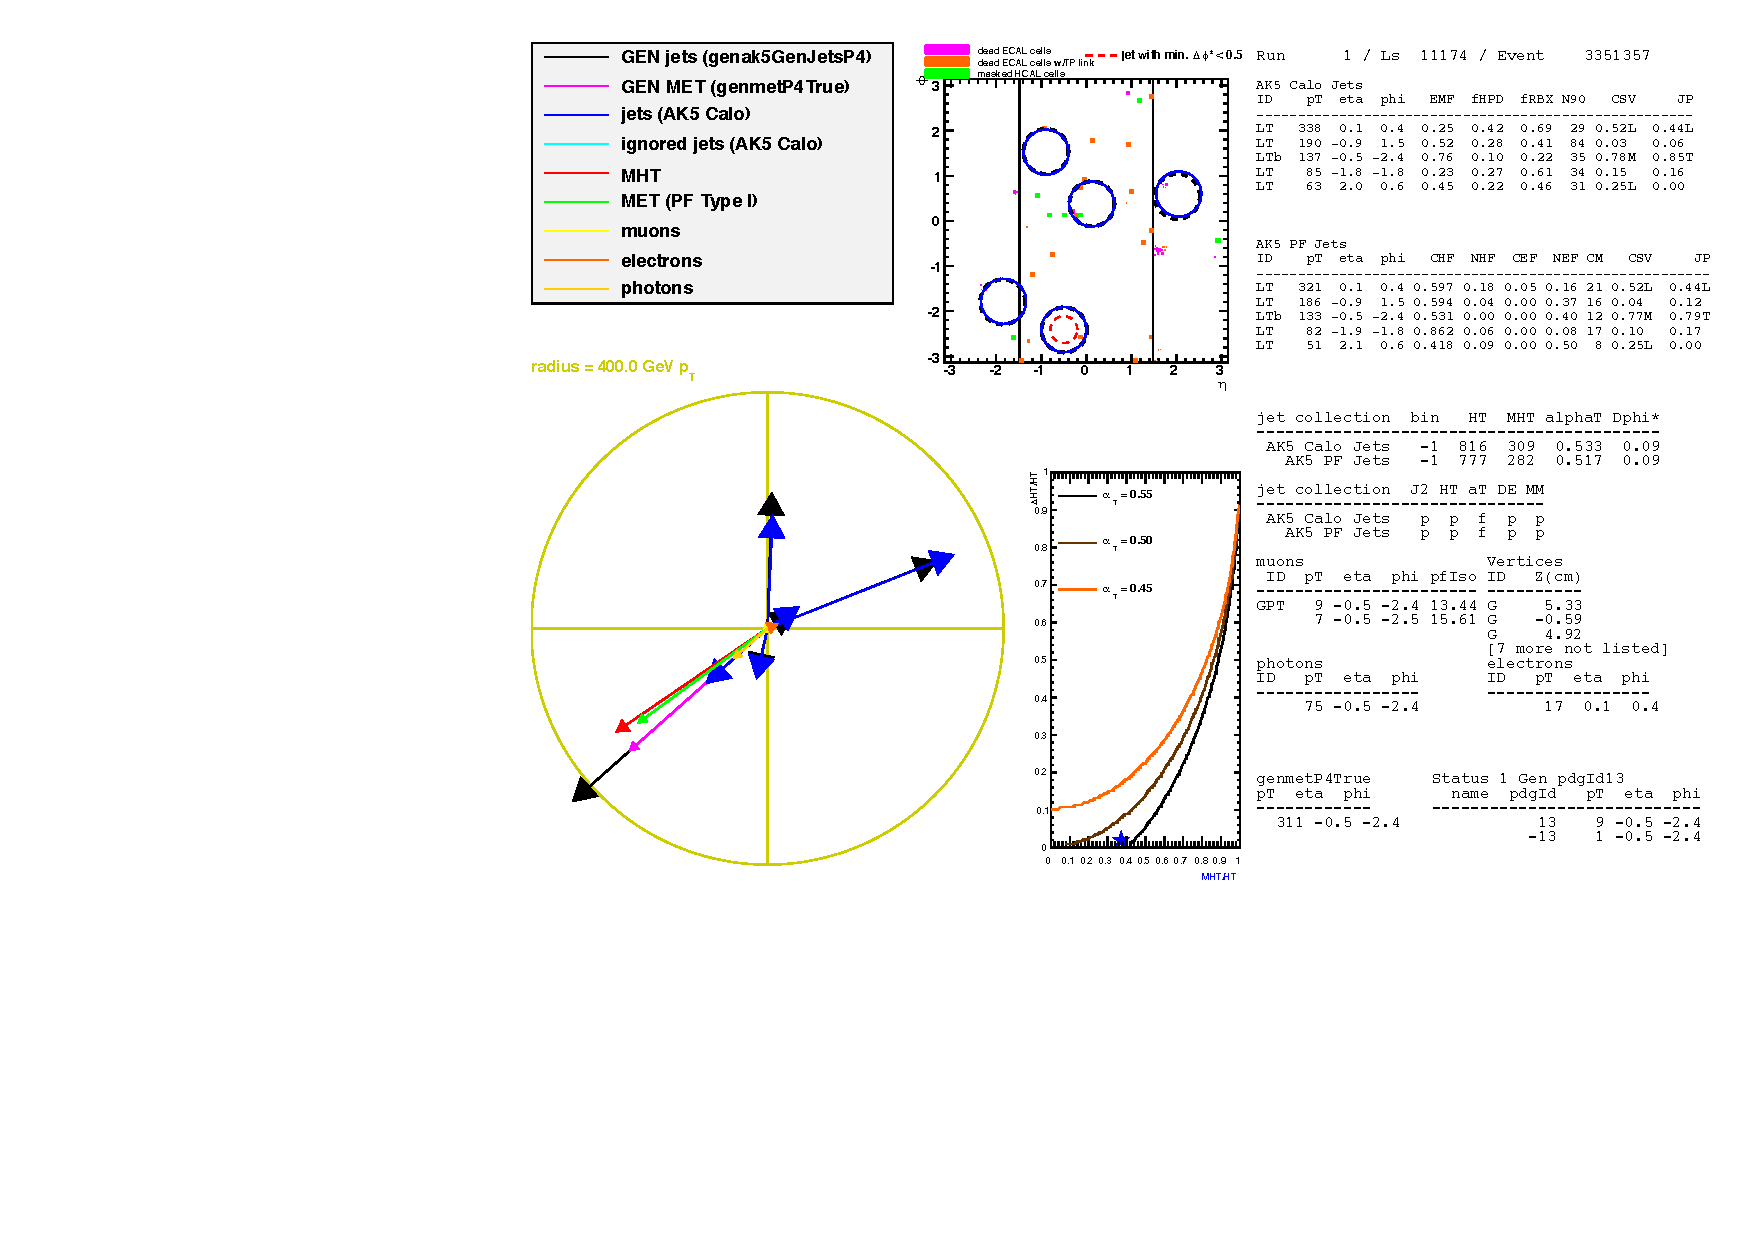
\includegraphics[width=\textwidth]
    {Figs/eventDisplays/Had_QCD_MG_MC_HT375_skim_displays_singleEvent.pdf}
    \caption{Event display blah}
    \label{fig:event_display_QCD}
\end{sidewaysfigure}
